\chapter{Contrôle du cycle cellulaire et mort cellulaire programmée}\label{ch:b3:cell-cycle-apoptosis}

Une centaine de milliards de cellules de votre corps mourront
aujourd'hui, exprès, et une centaine de milliards naîtront pour les
remplacer~; la paroi de votre intestin se renouvelle tous les cinq
jours, et vos globules rouges tous les quatre mois. Un têtard perd sa
queue sans saigner~; la palmure entre les doigts d'un embryon humain
disparaît à la huitième semaine~; la moitié des neurones jamais
produits dans un cerveau sont tués avant la naissance. Chacune de ces
morts est exécutée par la cellule elle-même, sur programme, et chacune
de ces naissances est autorisée par un système de contrôle qui décide,
en deux ou trois points du cycle, si la cellule a le droit de
continuer. Les deux programmes --- la division et le suicide --- font
l'objet de ce chapitre. Ils ont été démêlés chez la levure, dans des
œufs de grenouille, chez l'oursin et chez un ver qui possède exactement
$1090$ cellules somatiques dont exactement $131$ meurent, et ils se
sont révélés être les mêmes chez l'homme, où leurs défaillances sont le
cancer d'un côté et la dégénérescence de l'autre.

\section{Le moteur du cycle}

\begin{definition}[Cyclines et kinases dépendantes des cyclines]\label{def:b3:cell-cycle-apoptosis:cdk}
\index{cycline}\index{kinase dépendante des cyclines}\index{complexe promoteur de l'anaphase}\index{cycle cellulaire}
Le cycle cellulaire --- G1, S (réplication), G2, M (mitose) --- est
entraîné par une famille de protéines kinases, les \emph{kinases
dépendantes des cyclines} (CDK), dont les sous-unités catalytiques sont
présentes tout au long du cycle mais ne sont actives qu'une fois liées
à une \emph{cycline}, sous-unité régulatrice dont la concentration monte
et redescend dans un ordre fixe~: la cycline~D avec Cdk4/6 en G1 en
réponse aux facteurs de croissance, la cycline~E avec Cdk2 à la
transition G1/S, la cycline~A avec Cdk2 tout au long de la phase~S, la
cycline~B avec Cdk1 à l'entrée en mitose. Chaque couple cycline--CDK
phosphoryle les protéines de sa phase --- origines de réplication,
lamines, condensines, enzymes de l'assemblage du fuseau --- et chacun
est éteint par la destruction de sa cycline~: des ubiquitine-ligases
(SCF en G1/S, le \emph{complexe promoteur de l'anaphase}, APC/C, en
mitose) marquent les cyclines pour le protéasome. L'activité de Cdk1
est en outre commandée par une phosphorylation inhibitrice posée par la
kinase Wee1 et retirée par la phosphatase Cdc25, ainsi que par de
petites protéines inhibitrices (p21, p27, p16) qui se fixent sur les
complexes. Le cycle est donc une suite ordonnée de vagues de kinases,
chaque vague se terminant par la protéolyse de ce qui l'a produite.
\end{definition}

\begin{proof}[Faits expérimentaux]
Trois voies ont convergé. Hartwell (années 1970) a isolé des mutants
\emph{cdc} thermosensibles de la levure bourgeonnante, chacun arrêté à
un stade et reconnaissable à la taille de son bourgeon, et a défini le
\emph{Start}, le point de G1 au-delà duquel une cellule est engagée
dans un cycle. Nurse (années 1980) a trouvé chez la levure à fission
que \emph{cdc2} commandait le moment de la mitose et que le gène
humain, introduit dans la levure, sauvait le mutant~: la kinase était
Cdk1, conservée de la levure à l'homme. Hunt (1983) a trouvé dans des
œufs d'oursin une protéine qui s'accumulait à chaque cycle et était
brusquement détruite à chaque division, et l'a appelée \omterm{def:b3:cell-cycle-apoptosis:cdk}{cycline}. L'œuf
de grenouille avait entre-temps livré un «~facteur promoteur de la
maturation~» qui entraînait n'importe quel noyau en mitose~; c'était la
\omterm{def:b3:cell-cycle-apoptosis:cdk}{cycline}~B liée à Cdk1. Rao et Johnson (1970) avaient montré, en
fusionnant des cellules, qu'une cellule en phase~S entraîne un noyau G1
dans la réplication tandis qu'un noyau G2 attend --- le cytoplasme
porte le signal, et un noyau déjà répliqué ne peut pas être amené à se
répliquer de nouveau.
\end{proof}

\begin{omfigure}
\begin{tikzpicture}[every node/.style={font=\scriptsize}, >=stealth]
  % cycle circle with phases
  \draw[very thick, omDef!50] (0,0) circle (2.2);
  \foreach \a/\b/\col/\lab/\r in {90/200/omDef!25/G1/1.55, 200/270/omProp!30/S/1.55, 270/315/omMeth!30/G2/1.55, 315/450/omThm!30/M/1.55} {
    \fill[\col] (0,0) -- (\a:2.2) arc[start angle=\a, end angle=\b, radius=2.2] -- cycle;
    \node[font=\small\bfseries] at ({(\a+\b)/2}:\r) {\lab};
  }
  \fill[white] (0,0) circle (1.0);
  \draw[very thick, omDef!50] (0,0) circle (2.2);
  % cyclin-CDK labels around
  \node[left, align=right] at (-2.4,1.2) {cycline D--Cdk4/6\\facteurs de croissance, Rb éteinte};
  \node[left, align=right] at (-2.4,-1.0) {cycline E--Cdk2\\les origines démarrent};
  \node[anchor=north east, align=right] at (-1.3,-2.2) {cycline A--Cdk2\\réplication};
  \node[right, align=left] at (2.4,-1.0) {cycline B--Cdk1\\entrée en mitose};
  \node[right, align=left] at (2.4,1.3) {l'APC/C détruit la cycline B\\et la sécurine~: anaphase, sortie};
  % checkpoints as bars
  \foreach \a in {160,270,20} \draw[very thick, omThm] (\a:1.95) -- (\a:2.45);
  \node[align=center, anchor=south east] at (-1.2,2.35) {point de restriction~:\\facteurs de croissance~?};
  \node[align=left, anchor=west] at (2.55,0.35) {point de contrôle du fuseau~:\\tous les kinétochores attachés~?};
  \node[align=center, anchor=north] at (1.5,-2.55) {point de contrôle G2/M~:\\ADN intact~?};
  \draw[->, thick] (0,0) ++(60:1.25) arc[start angle=60, end angle=30, radius=1.25];
\end{tikzpicture}

{\small Le cycle comme suite de vagues cycline--CDK, chacune close par
la destruction de sa \omterm{def:b3:cell-cycle-apoptosis:cdk}{cycline}, avec les trois \omterm{def:b3:cell-cycle-apoptosis:checkpoints}{points de contrôle} (barres
rouges) où la cellule se demande s'il faut continuer.}
\end{omfigure}

\begin{theorem}[Un interrupteur et un frein retardé font un oscillateur]\label{thm:b3:cell-cycle-apoptosis:oscillator}
\index{oscillateur de relaxation}\index{bistabilité!cycle cellulaire}\index{hystérésis}
Soit $A$ l'activité du couple \omterm{def:b3:cell-cycle-apoptosis:cdk}{cycline}~B--Cdk1 et $C$ la quantité de
\omterm{def:b3:cell-cycle-apoptosis:cdk}{cycline}~B. Supposons (i) qu'à $C$ fixé, $A$ relaxe rapidement vers un
état stationnaire qui dépend de $C$ par une rétroaction positive (Cdk1
active active son activateur Cdc25 et inhibe son inhibiteur Wee1), de
sorte que la courbe stationnaire $A^{*}(C)$ est en S~: pour $C$ compris
entre deux seuils $C_{1} < C_{2}$ il existe à la fois un état bas et un
état haut, et le système reste sur la branche où il se trouve
(\emph{hystérésis})~; (ii) que $C$ varie lentement, synthétisée à la
vitesse constante $k_{s}$ et dégradée à la vitesse $k_{d}A\,C$ par
l'APC/C, que Cdk1 active allume après un délai. Alors le système n'a
aucun état stationnaire stable et exécute une \emph{oscillation de
relaxation}~: $C$ s'accumule sur la branche basse jusqu'à dépasser
$C_{2}$, $A$ saute sur la branche haute (entrée en mitose), la
dégradation dépasse la synthèse et $C$ chute jusqu'à passer sous
$C_{1}$, $A$ s'effondre sur la branche basse (sortie de mitose), et le
cycle recommence. La période est fixée surtout par la variable lente~:
environ $C_{2}/k_{s}$ pour la montée, plus le temps de dégradation de
$C_{2}$ à $C_{1}$.
\end{theorem}
\begin{proof}[Démonstration partielle]
Un état stationnaire du couple exigerait
$\mathrm{d}C/\mathrm{d}t = 0$, c'est-à-dire $k_{s} = k_{d}A^{*}(C)\,C$,
en un point de la courbe en S. Sur la branche basse $A^{*}$ est petit,
donc $k_{d}A^{*}C < k_{s}$ pour $C$ jusqu'à $C_{2}$~: la \omterm{def:b3:cell-cycle-apoptosis:cdk}{cycline} monte,
et le système est emporté hors du bout de la branche. Sur la branche
haute $A^{*}$ est grand, donc $k_{d}A^{*}C > k_{s}$ pour $C$ jusqu'à
$C_{1}$~: la \omterm{def:b3:cell-cycle-apoptosis:cdk}{cycline} baisse, et le système est emporté hors de ce
bout-là. Le seul état stationnaire candidat se trouverait sur la
branche intermédiaire, instable, et un point qui s'y trouve est
repoussé~; il n'existe donc aucun état stationnaire stable, et la
trajectoire, confinée aux deux branches stables et aux sauts entre
elles, tourne en rond. Le temps passé sur la branche basse vaut
$\int \mathrm{d}C/(k_{s} - k_{d}A^{*}C) \approx C_{2}/k_{s}$ quand
$A^{*}$ est petit, et le temps sur la branche haute est le temps plus
court qu'il faut pour dégrader $C_{2} - C_{1}$ à la vitesse
$k_{d}A^{*}_{\text{haut}}C$. L'existence de la courbe en S issue de la
rétroaction Cdc25/Wee1 est admise ici~; c'est la même bistabilité que
celle du gène auto-activateur du volume de deuxième année, la variable
rapide étant maintenant une kinase et la lente sa \omterm{def:b3:cell-cycle-apoptosis:cdk}{cycline}.
\end{proof}

\begin{omfigure}
\begin{tikzpicture}
\begin{axis}[
  width=6.6cm, height=5.6cm,
  axis lines=left,
  xmin=0, xmax=1.4, ymin=0, ymax=1.1,
  xlabel={cycline B, $C$}, ylabel={activité de Cdk1, $A$},
  xlabel style={font=\small, at={(axis description cs:0.5,-0.12)}, anchor=north}, ylabel style={font=\small},
  tick label style={font=\scriptsize}, xtick={0.4,1.0}, xticklabels={$C_{1}$,$C_{2}$}, ytick=\empty,
  clip=false,
]
% S-shaped nullcline: two stable branches and a dashed unstable one
\addplot[very thick, omDef, smooth] coordinates {(0,0.02) (0.5,0.04) (0.9,0.07) (1.0,0.1)};
\addplot[very thick, omDef, dashed, smooth] coordinates {(1.0,0.1) (0.85,0.3) (0.7,0.5) (0.55,0.7) (0.4,0.9)};
\addplot[very thick, omDef, smooth] coordinates {(0.4,0.9) (0.6,0.94) (1.0,0.97) (1.4,0.98)};
\draw[->, very thick, omThm] (axis cs:0.05,0.15) -- (axis cs:0.98,0.15);
\draw[->, very thick, omThm] (axis cs:1.04,0.18) -- (axis cs:1.04,0.82);
\draw[->, very thick, omThm] (axis cs:0.98,0.84) -- (axis cs:0.42,0.84);
\draw[->, very thick, omThm] (axis cs:0.36,0.82) -- (axis cs:0.36,0.18);
\node[font=\scriptsize, omThm, anchor=south west] at (axis cs:0.36,0.24) {la cycline s'accumule};
\node[font=\scriptsize, omThm, anchor=west] at (axis cs:1.07,0.5) {entrée};
\node[font=\scriptsize, omThm, anchor=south] at (axis cs:0.7,1.0) {l'APC/C dégrade la cycline (mitose)};
\node[font=\scriptsize, omThm, anchor=east] at (axis cs:0.33,0.5) {sortie};
\node[font=\scriptsize, omDef, anchor=north east] at (axis cs:1.38,0.95) {$A^{*}(C)$};
\end{axis}
\begin{axis}[
  at={(7.6cm,0)}, anchor=south west,
  width=6.6cm, height=5.6cm,
  axis lines=left,
  xmin=0, xmax=3, ymin=0, ymax=1.2,
  xlabel={temps (cycles)}, ylabel={},
  xlabel style={font=\small, at={(axis description cs:0.5,-0.12)}, anchor=north},
  tick label style={font=\scriptsize}, xtick={0,1,2,3}, ytick=\empty,
  clip=false,
]
\addplot[very thick, omDef] coordinates {(0,0.4) (0.8,1.0) (0.95,0.4) (1.75,1.0) (1.9,0.4) (2.7,1.0) (2.85,0.4) (3,0.5)};
\addplot[very thick, omThm] coordinates {(0,0.05) (0.8,0.05) (0.8,0.95) (0.95,0.95) (0.95,0.05) (1.75,0.05) (1.75,0.95) (1.9,0.95) (1.9,0.05) (2.7,0.05) (2.7,0.95) (2.85,0.95) (2.85,0.05) (3,0.05)};
\node[font=\scriptsize, omDef, anchor=south west] at (axis cs:1.0,0.1) {cycline B};
\node[font=\scriptsize, omThm, anchor=south west] at (axis cs:1.0,1.0) {activité de Cdk1};
\end{axis}
\end{tikzpicture}

{\small À gauche~: le plan de phase de l'oscillateur. La courbe en S est
l'état stationnaire rapide de Cdk1 pour chaque niveau de \omterm{def:b3:cell-cycle-apoptosis:cdk}{cycline}~; la
boucle rouge est le cycle --- accumulation lente le long de la branche
basse, saut en $C_{2}$, dégradation rapide le long de la branche haute,
saut de retour en $C_{1}$. À droite~: l'évolution temporelle qui en
résulte, une dent de scie de \omterm{def:b3:cell-cycle-apoptosis:cdk}{cycline} et un créneau de kinase.}
\end{omfigure}

\begin{example}[Pourquoi l'œuf de grenouille est une horloge]\label{ex:b3:cell-cycle-apoptosis:frog}
Un œuf de grenouille fécondé se divise douze fois en six heures, sans
croissance, sans transcription et sans \omterm{def:b3:cell-cycle-apoptosis:checkpoints}{points de contrôle}, à
intervalles de \qty{30}{min}~: c'est l'oscillateur du théorème tournant
à nu, et un extrait de son cytoplasme dans un tube à essai continue de
cycler, la \omterm{def:b3:cell-cycle-apoptosis:cdk}{cycline} montant et redescendant, sans rien à diviser.
Ajouter une \omterm{def:b3:cell-cycle-apoptosis:cdk}{cycline}~B non dégradable bloque l'extrait en mitose,
puisque $C$ ne peut jamais tomber sous $C_{1}$~; bloquer la synthèse de
\omterm{def:b3:cell-cycle-apoptosis:cdk}{cycline} le bloque en interphase. Dans une cellule somatique, le même
moteur est enveloppé dans les contrôles de la section suivante, qui le
retiennent aux seuils jusqu'à ce que les conditions soient remplies, de
sorte que la période devient un jour plutôt qu'une demi-heure et peut
s'allonger indéfiniment.
\end{example}

\section{Les points de contrôle}

\begin{definition}[Les points de contrôle]\label{def:b3:cell-cycle-apoptosis:checkpoints}
\index{point de contrôle}\index{point de restriction}\index{point de contrôle de l'assemblage du fuseau}\index{autorisation de réplication}
Un \emph{point de contrôle} est un dispositif qui arrête le cycle à une
transition jusqu'à ce qu'une condition soit remplie, en agissant sur le
moteur --- en inhibant une CDK ou une ubiquitine-ligase. Trois comptent
plus que les autres. Le \emph{point de restriction} de la fin de G1 (le
Start chez la levure)~: la cellule ne continue que si les facteurs de
croissance, les nutriments et la taille le permettent~; au-delà, le
cycle s'achève sans eux. Le \emph{point de contrôle G2/M}~: un ADN lésé
ou non répliqué, signalé par les kinases \omterm{def:b3:dna-repair:ddr}{ATM}/ATR du
\cref{ch:b3:dna-repair}, maintient Cdc25 inhibée et donc Cdk1
phosphorylée et inactive. Le \emph{point de contrôle de l'assemblage du
fuseau}~: un seul kinétochore non attaché aux \omterm{def:b3:cytoskeleton-motility:filaments}{microtubules} produit un
inhibiteur diffusible (Mad2 lié à Cdc20) qui maintient l'APC/C éteint,
de sorte que l'anaphase attend le dernier chromosome. Un quatrième
contrôle ne comporte aucune attente mais est tout aussi strict~:
l'\emph{autorisation de réplication}. Les origines ne sont chargées de
l'hélicase MCM qu'en G1, quand l'activité CDK est faible, et les
facteurs de chargement sont détruits ou inhibés dès que la phase~S
commence, de sorte que chaque origine démarre une fois et une seule par
cycle --- la raison pour laquelle un noyau G2 des fusions de Rao et
Johnson ne pouvait pas être amené à se répliquer.
\end{definition}

\begin{proposition}[Le point de restriction est un interrupteur]\label{prop:b3:cell-cycle-apoptosis:rb}
\index{protéine du rétinoblastome}\index{E2F}
Au début de G1, le facteur de transcription \emph{E2F}, qui commande
les gènes de la phase~S (\omterm{def:b3:cell-cycle-apoptosis:cdk}{cycline}~E, \omterm{def:b3:cell-cycle-apoptosis:cdk}{cycline}~A, enzymes de la
réplication), est maintenu inactif par la \emph{\omterm{prop:b3:cell-cycle-apoptosis:rb}{protéine du
rétinoblastome}} Rb. Les facteurs de croissance induisent la \omterm{def:b3:cell-cycle-apoptosis:cdk}{cycline}~D,
et le couple \omterm{def:b3:cell-cycle-apoptosis:cdk}{cycline}~D--Cdk4/6 commence à phosphoryler Rb, ce qui
libère un peu d'E2F~; E2F induit alors la \omterm{def:b3:cell-cycle-apoptosis:cdk}{cycline}~E, et le couple
\omterm{def:b3:cell-cycle-apoptosis:cdk}{cycline}~E--Cdk2 phosphoryle Rb bien davantage --- une rétroaction
positive qui, une fois un seuil franchi, s'achève sans autre facteur de
croissance. La cellule a franchi le \omterm{def:b3:cell-cycle-apoptosis:checkpoints}{point de restriction}~; E2F induit
aussi son propre gène. La perte de Rb, ou de l'inhibiteur de Cdk4/6
p16, ou l'amplification de la \omterm{def:b3:cell-cycle-apoptosis:cdk}{cycline}~D, supprime toute exigence de
facteur de croissance, et chacune est fréquente dans les cancers
(\cref{ch:b3:cancer-biology})~; des médicaments qui inhibent Cdk4/6
sont aujourd'hui employés contre les cancers du sein qui dépendent de
cet interrupteur.
\end{proposition}

\begin{omfigure}
\begin{tikzpicture}[every node/.style={font=\scriptsize}, >=stealth]
  \node[draw, thick, rounded corners, fill=omProp!25, minimum width=2.2cm] (gf) at (0,2.2) {facteurs de croissance};
  \node[draw, thick, rounded corners, fill=omDef!20, minimum width=2.4cm] (cd) at (0,1.0) {cycline D--Cdk4/6};
  \node[draw, thick, rounded corners, fill=omThm!20, minimum width=1.6cm] (rb) at (3.8,1.0) {Rb};
  \node[draw, thick, rounded corners, fill=omMeth!25, minimum width=1.6cm] (e2f) at (7.2,1.0) {E2F};
  \node[draw, thick, rounded corners, fill=omDef!20, minimum width=2.4cm] (ce) at (7.2,-0.6) {cycline E--Cdk2};
  \node[draw, thick, rounded corners, fill=gray!15, align=center, minimum width=2.6cm] (s) at (10.8,1.0) {gènes de la phase S~:\\cycline A, MCM, \dots};
  \draw[->, thick] (gf) -- (cd);
  \draw[-|, thick, omThm] (cd) -- (rb) node[midway, above, font=\tiny] {phosphoryle};
  \draw[-|, thick, omThm] (rb) -- (e2f) node[midway, above, font=\tiny] {maintient inactif};
  \draw[->, thick] (e2f) -- (s);
  \draw[->, thick] (e2f) -- (ce) node[midway, right] {induit};
  \draw[-|, thick, omThm] (ce.west) -- ++(-2.2,0) |- (rb.south) node[pos=0.25, below] {phosphoryle Rb davantage};
  \draw[->, thick, omMeth!70!black] (e2f.north) .. controls (6.0,2.2) and (6.8,2.2) .. (e2f.north east) node[pos=0.5, above] {induit son propre gène};
  \node[draw, thick, rounded corners, fill=omThm!10] (p16) at (0,-0.6) {p16}; \draw[-|, thick, omThm] (p16) -- (cd);
\end{tikzpicture}

{\small Le \omterm{def:b3:cell-cycle-apoptosis:checkpoints}{point de restriction}. Les facteurs de croissance amorcent la
phosphorylation de Rb, qui libère un peu d'E2F~; E2F induit la
\omterm{def:b3:cell-cycle-apoptosis:cdk}{cycline}~E, dont la kinase phosphoryle Rb davantage --- une rétroaction
positive qui achève la transition et la rend indépendante du signal
initial. Les barres marquent l'inhibition.}
\end{omfigure}

\begin{proposition}[L'anaphase est une décision protéolytique]\label{prop:b3:cell-cycle-apoptosis:anaphase}
\index{sécurine}\index{séparase}\index{cohésine}
Les chromatides sœurs sont tenues ensemble depuis la phase~S par des
anneaux de \emph{cohésine}. En métaphase, quand chaque kinétochore est
attaché et que le \omterm{def:b3:cell-cycle-apoptosis:checkpoints}{point de contrôle} du fuseau est éteint, l'APC/C avec
son activateur Cdc20 ubiquitinyle deux protéines~: la \omterm{def:b3:cell-cycle-apoptosis:cdk}{cycline}~B, dont
la perte inactive Cdk1 et permet à la cellule de sortir de mitose, et
la \emph{sécurine}, dont la perte libère la protéase \emph{séparase},
qui coupe la cohésine. Toutes les paires de sœurs se séparent à
quelques secondes les unes des autres, tirées vers les pôles par le
fuseau, et la cellule se divise par un anneau d'actine et de \omterm{def:b3:cytoskeleton-motility:motors}{myosine}~II
assemblé là où la zone médiane du fuseau l'indique au cortex (par
RhoA). La décision est irréversible parce qu'elle est protéolytique~:
une cohésine coupée ne se réassemble pas, et la \omterm{def:b3:cell-cycle-apoptosis:cdk}{cycline} dégradée doit
être resynthétisée. Les erreurs commises ici --- un chromosome tiré
vers le mauvais pôle, une anaphase commencée avant le dernier
attachement --- produisent des filles aneuploïdes, l'anomalie
chromosomique la plus fréquente des tumeurs et des fausses couches.
\end{proposition}

\begin{omfigure}
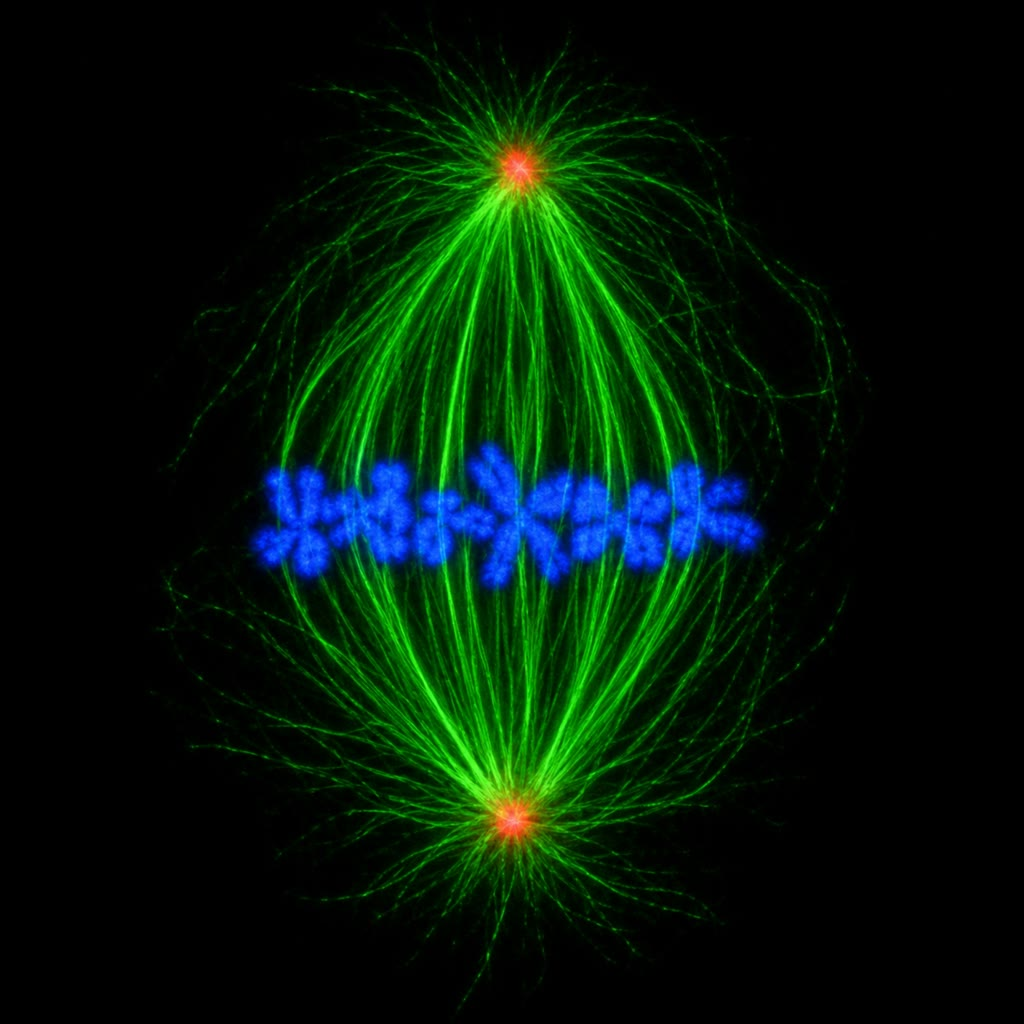
\includegraphics[width=0.36\linewidth]{images/book5/ai/b5-10-mitotic-spindle.jpg}\hspace{0.04\linewidth}
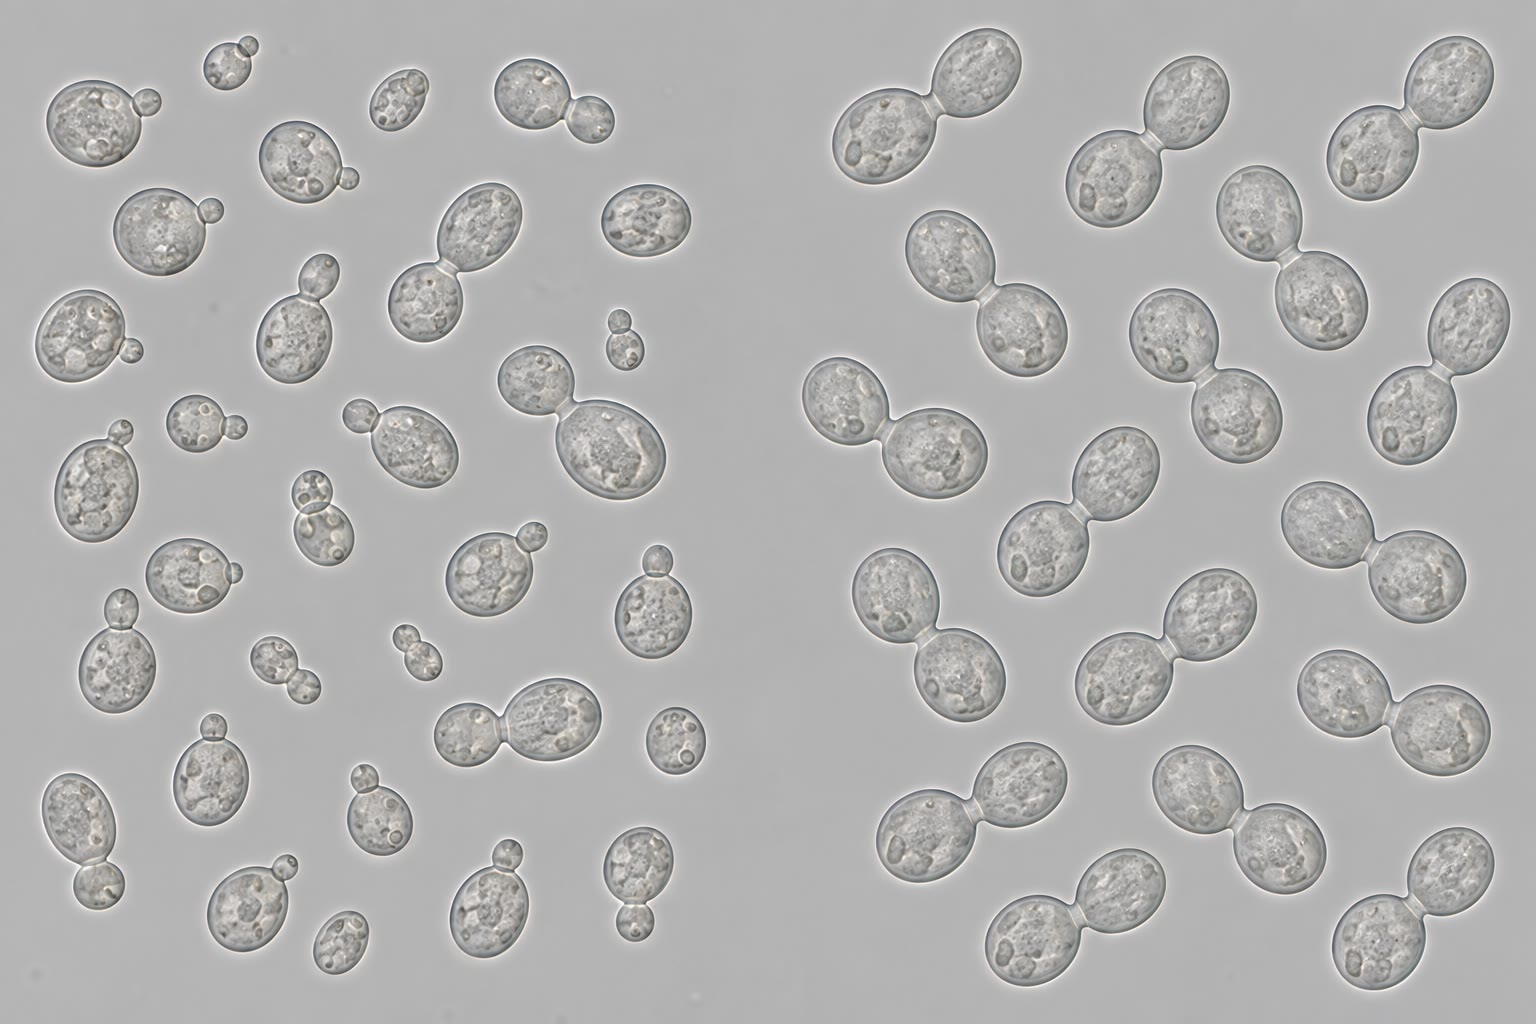
\includegraphics[width=0.54\linewidth]{images/book5/ai/b5-10-yeast-cdc-mutants.jpg}

{\small À gauche~: une cellule en métaphase --- les \omterm{def:b3:cytoskeleton-motility:filaments}{microtubules} du
fuseau (vert) issus des deux pôles (rouge), les chromosomes (bleu)
alignés sur la plaque, l'instant où le \omterm{def:b3:cell-cycle-apoptosis:checkpoints}{point de contrôle} du fuseau
décide. À droite~: la levure bourgeonnante, type sauvage avec des
bourgeons de toutes tailles (à gauche) et un mutant \emph{cdc} où
chaque cellule s'est arrêtée au même stade, chacune avec un bourgeon de
même taille (à droite).}
\end{omfigure}

\section{L'apoptose}

\begin{definition}[L'apoptose]\label{def:b3:cell-cycle-apoptosis:apoptosis}
\index{apoptose}\index{nécrose}\index{caspase}\index{phosphatidylsérine}
L'\emph{apoptose} est la mort cellulaire programmée par une séquence
intrinsèque~: la cellule se rétracte et s'arrondit, sa \omterm{def:b3:chromatin-epigenetics:nucleosome}{chromatine} se
condense et son ADN est coupé entre les \omterm{def:b3:chromatin-epigenetics:nucleosome}{nucléosomes} en une échelle de
fragments, le noyau se fragmente, la membrane bourgeonne en vésicules
closes, la phosphatidylsérine apparaît sur la face externe de la
membrane comme un signal «~mangez-moi~», et les fragments sont englobés
par les voisines ou par des macrophages en moins d'une heure --- sans
fuite, et donc sans inflammation. Elle est exécutée par des
\emph{caspases}, protéases à cystéine qui coupent après un aspartate et
sont produites sous forme de zymogènes inactifs~: les caspases
\emph{initiatrices} (8 et 9) sont activées par leur rassemblement sur
une plate-forme, et elles clivent et activent les caspases
\emph{exécutrices} (3 et 7), qui coupent plusieurs centaines de
substrats --- les lamines, le cytosquelette, l'inhibiteur de la
nucléase qui coupe l'ADN, l'enzyme qui garde la phosphatidylsérine à
l'intérieur. La \emph{nécrose}, à l'inverse, est une mort par lésion~:
la cellule gonfle, éclate, répand son contenu et provoque une
inflammation. L'apoptose a été nommée et sa morphologie décrite par
Kerr, Wyllie et Currie (1972)~; ses gènes ont été trouvés chez un ver.
\end{definition}

\begin{proof}[Faits expérimentaux]
Chaque hermaphrodite de \emph{Caenorhabditis elegans} produit $1090$
cellules somatiques, dont les mêmes $131$ meurent, chacune à un moment
et à un endroit fixés. Horvitz et ses collègues (années 1980) ont isolé
des mutants où elles survivaient~: \emph{ced-3} et \emph{ced-4} étaient
nécessaires à toutes les morts, et en leur absence les $131$ cellules
vivaient et se différenciaient~; \emph{ced-9} protégeait --- sa perte
tuait des cellules qui auraient dû vivre, son excès d'activité sauvait
des cellules qui auraient dû mourir~; \emph{egl-1} était nécessaire à
certaines morts. CED-3 était une \omterm{def:b3:cell-cycle-apoptosis:apoptosis}{caspase}, CED-4 sa plate-forme
d'activation (Apaf-1 chez l'homme), CED-9 une protéine Bcl-2, EGL-1 une
protéine à BH3 seul~: la voie humaine, gène pour gène. Le gène humain
\emph{BCL2} avait lui-même été trouvé à une translocation
chromosomique dans le lymphome folliculaire, cancer de cellules qui ne
meurent pas.
\end{proof}

\begin{definition}[Les deux voies]\label{def:b3:cell-cycle-apoptosis:pathways}
\index{voie intrinsèque}\index{voie extrinsèque}\index{famille Bcl-2}\index{cytochrome c}\index{apoptosome}\index{récepteur de mort}
La voie \emph{intrinsèque} (mitochondriale) intègre l'état interne de
la cellule. La \emph{famille Bcl-2} compte trois classes~: les gardiens
(Bcl-2, Bcl-xL, Mcl-1), qui siègent sur la membrane externe
mitochondriale et la maintiennent close~; les effecteurs (Bax, Bak),
qui s'oligomérisent en pores dans cette membrane une fois activés~; et
les capteurs \emph{à BH3 seul} (Bim, Bid, Puma, Noxa, Bad), chacun
induit ou activé par une agression particulière --- \omterm{def:b3:dna-repair:lesions}{lésion de l'ADN} par
p53 (Puma, Noxa), retrait d'un facteur de croissance (Bim, Bad),
détachement, protéines mal repliées --- et qui se fixent aux gardiens
et libèrent ou activent les effecteurs. Quand les effecteurs
l'emportent, la membrane externe est perméabilisée, le
\emph{cytochrome~c} fuit dans le cytosol, se lie à Apaf-1 et forme
l'\emph{apoptosome}, qui active la \omterm{def:b3:cell-cycle-apoptosis:apoptosis}{caspase}~9. La voie
\emph{extrinsèque} commence au dehors~: des \emph{récepteurs de mort}
(Fas, récepteur du TNF, récepteurs de TRAIL), liés par leurs ligands
portés par un lymphocyte tueur ou une cellule voisine, se regroupent,
recrutent des adaptateurs et activent la \omterm{def:b3:cell-cycle-apoptosis:apoptosis}{caspase}~8, qui clive
directement la \omterm{def:b3:cell-cycle-apoptosis:apoptosis}{caspase}~3 et, par Bid, ouvre aussi la route
mitochondriale. Les deux voies convergent sur les \omterm{def:b3:cell-cycle-apoptosis:apoptosis}{caspases} exécutrices,
et des protéines inhibitrices (IAP, FLIP) en règlent le seuil au
passage.
\end{definition}

\begin{omfigure}
\begin{tikzpicture}[every node/.style={font=\scriptsize}, >=stealth]
  % extrinsic
  \node[draw, thick, rounded corners, fill=omProp!25, align=center] (lig) at (0,4.2) {ligand de mort sur une cellule tueuse\\(FasL, TNF, TRAIL)};
  \node[draw, thick, rounded corners, fill=omProp!25, align=center] (rec) at (0,2.8) {les récepteurs de mort se regroupent~;\\des adaptateurs recrutent la caspase-8};
  \node[draw, thick, rounded corners, fill=omThm!20] (c8) at (0,1.5) {caspase-8 active};
  % intrinsic
  \node[draw, thick, rounded corners, fill=omDef!20, align=center] (insult) at (7.2,4.2) {lésion de l'ADN (p53), perte d'un facteur,\\détachement, protéines mal repliées};
  \node[draw, thick, rounded corners, fill=omDef!20, align=center] (bh3) at (7.2,3.0) {les capteurs à BH3 seul (Puma, Bim, Bid)\\neutralisent Bcl-2, activent Bax/Bak};
  \node[draw, thick, rounded corners, fill=omDef!20, align=center] (mito) at (7.2,1.7) {la membrane externe s'ouvre~:\\le cytochrome $c$ sort, l'apoptosome se forme};
  \node[draw, thick, rounded corners, fill=omThm!20] (c9) at (7.2,0.5) {caspase-9 active};
  % convergence
  \node[draw, thick, rounded corners, fill=omThm!35, align=center] (c3) at (3.6,-0.8) {caspases exécutrices 3 et 7~:\\des centaines de substrats coupés};
  \node[draw, thick, rounded corners, fill=gray!15, align=center] (out) at (3.6,-2.3) {chromatine condensée, ADN en échelle, bourgeonnement,\\phosphatidylsérine exposée, corps englobés};
  \draw[->, thick] (lig) -- (rec); \draw[->, thick] (rec) -- (c8); \draw[->, thick] (c8) -- (c3);
  \draw[->, thick] (insult) -- (bh3); \draw[->, thick] (bh3) -- (mito); \draw[->, thick] (mito) -- (c9); \draw[->, thick] (c9) -- (c3);
  \draw[->, thick] (c3) -- (out);
  \draw[->, thick, dashed] (c8) -- (bh3) node[pos=0.55, below, sloped] {Bid clivée~: les deux routes se rejoignent};
  \node[left, omThm, align=right] at (-2.3,1.5) {voie\\extrinsèque}; \node[right, omDef, align=left] at (10.4,1.7) {voie\\intrinsèque};
  \node[right, font=\tiny, align=left] at (8.6,0.5) {les IAP inhibent ici~;\\Bcl-2 garde au-dessus};
\end{tikzpicture}

{\small Les deux routes vers les \omterm{def:b3:cell-cycle-apoptosis:apoptosis}{caspases} exécutrices. Du dehors vers le
dedans, un \omterm{def:b3:cell-cycle-apoptosis:pathways}{récepteur de mort} active la caspase-8~; du dedans vers le
dehors, la \omterm{def:b3:cell-cycle-apoptosis:pathways}{famille Bcl-2} pèse l'état de la cellule et, quand les
effecteurs l'emportent, la mitochondrie libère le cytochrome~$c$ et la
caspase-9 est activée. Les deux convergent sur la caspase-3.}
\end{omfigure}

\begin{proposition}[Le point de non-retour]\label{prop:b3:cell-cycle-apoptosis:mompt}
\index{perméabilisation de la membrane externe mitochondriale}
La \omterm{prop:b3:cell-cycle-apoptosis:mompt}{perméabilisation de la membrane externe mitochondriale} est soudaine
--- toutes les mitochondries d'une cellule s'ouvrent en cinq minutes
environ, après des heures de délibération --- et complète~: une fois le
cytochrome~$c$ dans le cytosol, l'activation des \omterm{def:b3:cell-cycle-apoptosis:apoptosis}{caspases} suit en
quelques minutes et ne peut plus être défaite en retirant le stimulus.
Deux traits en font un interrupteur. Le pore Bax/Bak se forme par
oligomérisation, de sorte que sa vitesse de formation croît fortement
avec la quantité d'effecteur activé~; et les gardiens et les capteurs
se lient les uns aux autres avec une forte affinité, de sorte que
jusqu'à un seuil chaque capteur est neutralisé et qu'au-delà chaque
capteur supplémentaire est libre --- un titrage, comme un tampon qui
s'épuise. La cellule ne meurt donc pas graduellement~; elle accumule
des protéines à BH3 seul jusqu'au franchissement d'un seuil, puis meurt
d'un coup. Les médicaments qui imitent les protéines BH3 (le
vénétoclax, qui occupe Bcl-2) font franchir ce seuil aux cellules déjà
«~amorcées~» --- proches du seuil, comme le sont beaucoup de cellules
leucémiques --- en épargnant celles qui ne le sont pas.
\end{proposition}

\begin{omfigure}
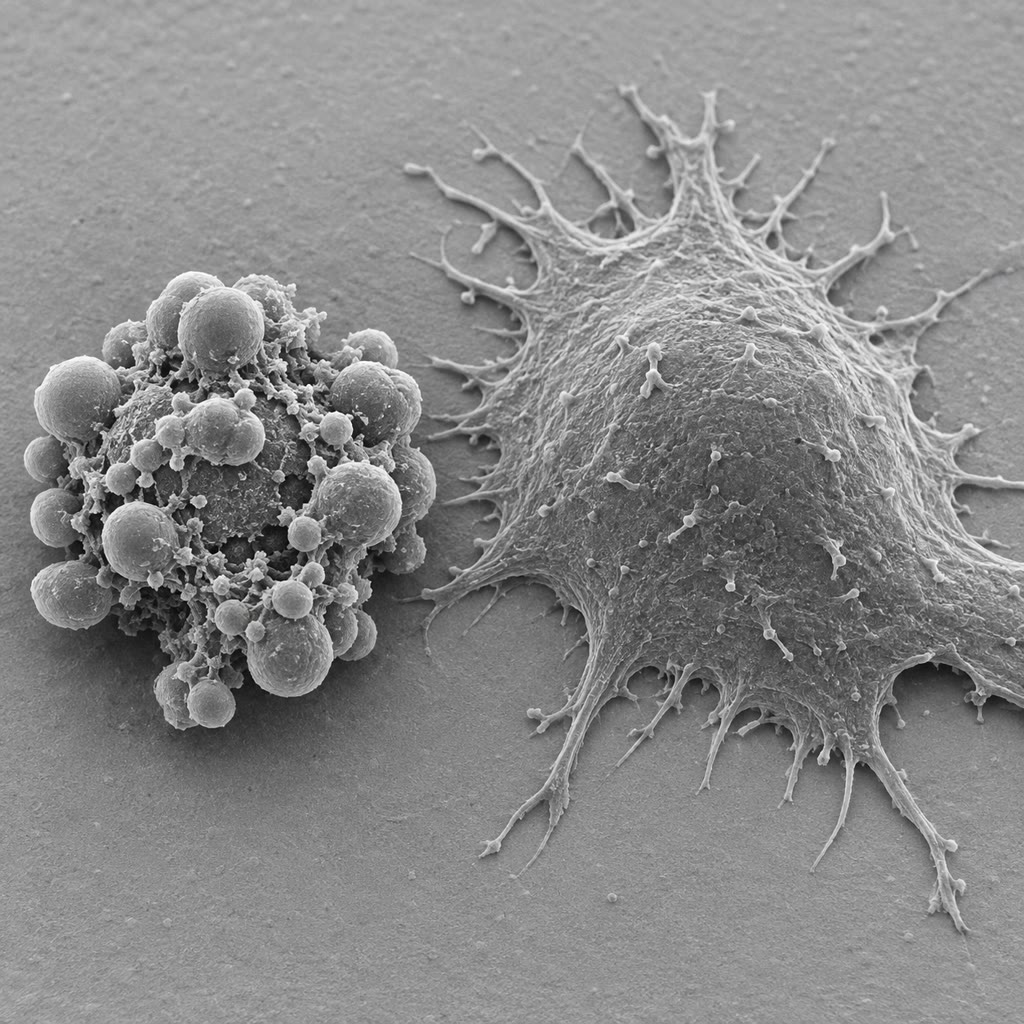
\includegraphics[width=0.40\linewidth]{images/book5/ai/b5-10-apoptotic-cell.jpg}

{\small Une cellule apoptotique à côté d'une cellule saine, au
microscope électronique à balayage~: rétractée, sa surface brisée en
bourgeons clos qui seront englobés sans la moindre trace
d'inflammation.}
\end{omfigure}

\begin{example}[Des morts qui bâtissent un corps]\label{ex:b3:cell-cycle-apoptosis:development}
Les doigts sont sculptés dans une palette par l'\omterm{def:b3:cell-cycle-apoptosis:apoptosis}{apoptose} des cellules
qui les séparent~; chez le canard ces mêmes cellules vivent et la
palmure demeure. La queue du têtard est résorbée à la métamorphose sur
le signal de l'hormone thyroïdienne. Environ la moitié des neurones
produits dans le système nerveux des vertébrés meurent avant la
naissance, ceux qui ne reçoivent pas assez de facteur trophique de
leurs cibles --- une compétition qui ajuste le nombre de neurones à la
taille du champ qu'ils desservent. Quatre-vingt-quinze pour cent des
lymphocytes~T produits dans le thymus y meurent, éliminés par sélection
parce qu'ils ne reconnaissent rien ou reconnaissent le soi
(\cref{ch:b3:adaptive-immunity}). Et chaque jour l'épithélium
intestinal laisse tomber ses cellules les plus vieilles au sommet des
villosités, la peau ses kératinocytes, le sang ses neutrophiles âgés
après une vie d'un jour~: l'\omterm{def:b3:cell-cycle-apoptosis:apoptosis}{apoptose} est la routine, et la taille d'un
tissu est la différence entre deux grandes vitesses.
\end{example}

\section{D'autres sorties, et l'échec de la sortie}

\begin{definition}[Nécroses régulées et sénescence]\label{def:b3:cell-cycle-apoptosis:other}
\index{nécroptose}\index{pyroptose}\index{sénescence}
Les cellules disposent d'autres morts programmées, toutes
inflammatoires là où l'\omterm{def:b3:cell-cycle-apoptosis:apoptosis}{apoptose} est silencieuse. La
\emph{nécroptose}, déclenchée par les \omterm{def:b3:cell-cycle-apoptosis:pathways}{récepteurs de mort} quand la
caspase-8 est bloquée (comme la bloquent certains virus), assemble la
kinase RIPK3 avec MLKL, qui perce la membrane plasmique. La
\emph{pyroptose}, dans les macrophages infectés, est exécutée par la
caspase-1 de l'inflammasome (\cref{ch:b3:innate-immunity}), qui clive
la gasdermine en un formeur de pores et libère l'interleukine-1. La
\emph{ferroptose} est une mort par peroxydation lipidique dépendante du
fer. Une cellule peut aussi cesser de se diviser sans mourir~: la
\emph{sénescence} est un arrêt définitif, imposé par p16 et p21 après
l'érosion des télomères (\cref{ch:b3:stem-cells}), une lésion
persistante de l'ADN ou l'activation d'un oncogène, et dans lequel la
cellule reste métaboliquement active et sécrète des facteurs
inflammatoires. La sénescence retire du pool de division les cellules
abîmées --- un suppresseur de tumeur --- et s'accumule avec l'âge, où
ses sécrétions contribuent à la dégénérescence des tissus~; éliminer
les cellules sénescentes chez la souris allonge la vie en bonne santé.
\end{definition}

\begin{remark}[Trop peu et trop]\label{rem:b3:cell-cycle-apoptosis:disease}
Les maladies de ces programmes sont des maladies de dose. Trop peu de
mort~: le cancer, où le seuil apoptotique est relevé par la
surexpression de Bcl-2 ou la perte de p53, de sorte que des cellules au
génome abîmé survivent et accumulent d'autres dégâts~; l'auto-immunité,
quand des lymphocytes qui auraient dû mourir à la sélection persistent.
Trop de mort~: la perte des lymphocytes~T dans l'infection par le VIH,
les neurones de la pénombre d'un accident vasculaire qui meurent par
\omterm{def:b3:cell-cycle-apoptosis:apoptosis}{apoptose} des heures après l'ischémie (une fenêtre pour traiter),
l'\omterm{def:b3:cell-cycle-apoptosis:apoptosis}{apoptose} lente des neurones dans les maladies neurodégénératives, les
cellules cardiaques perdues après un infarctus. Le traitement du cancer
est en grande partie l'induction délibérée de l'\omterm{def:b3:cell-cycle-apoptosis:apoptosis}{apoptose} dans des
cellules dont les seuils sont plus bas que ceux de leurs voisines, et
les médicaments qui visent Bcl-2 et Cdk4/6 sont les premiers conçus
d'après les cartes de ce chapitre.
\end{remark}

\section{Exercices}

\begin{exercise}[$\star$]\label{exo:b3:cell-cycle-apoptosis:1}
Énumérer les quatre phases du cycle, le couple cycline--CDK qui
commande chaque transition, et l'ubiquitine-ligase qui met fin à la
mitose.
\end{exercise}

\begin{exercise}[$\star$]\label{exo:b3:cell-cycle-apoptosis:2}
Qu'a apporté chacun de Hartwell, Nurse et Hunt à la découverte du
moteur, et chez quel organisme~?
\end{exercise}

\begin{exercise}[$\star$]\label{exo:b3:cell-cycle-apoptosis:3}
Nommer les trois \omterm{def:b3:cell-cycle-apoptosis:checkpoints}{points de contrôle}, la condition que chacun teste et
la cible moléculaire sur laquelle chacun agit.
\end{exercise}

\begin{exercise}[$\star$]\label{exo:b3:cell-cycle-apoptosis:4}
Distinguer l'\omterm{def:b3:cell-cycle-apoptosis:apoptosis}{apoptose} de la \omterm{def:b3:cell-cycle-apoptosis:apoptosis}{nécrose} par cinq traits, et nommer la
classe d'enzymes qui exécute l'\omterm{def:b3:cell-cycle-apoptosis:apoptosis}{apoptose}.
\end{exercise}

\begin{exercise}[$\star\star$]\label{exo:b3:cell-cycle-apoptosis:5}
Dans un extrait d'œuf de grenouille, la \omterm{def:b3:cell-cycle-apoptosis:cdk}{cycline}~B est synthétisée à
$k_{s} = 1$ unité par minute~; le seuil mitotique est $C_{2} = 30$
unités, le seuil de sortie $C_{1} = 5$, et en mitose la \omterm{def:b3:cell-cycle-apoptosis:cdk}{cycline} est
dégradée avec une demi-vie de \qty{2}{min}. Estimer la période de
l'oscillation et la fraction du cycle passée en mitose.
\end{exercise}

\begin{exercise}[$\star\star$]\label{exo:b3:cell-cycle-apoptosis:6}
Prévoir le comportement d'une cellule (a) qui exprime une \omterm{def:b3:cell-cycle-apoptosis:cdk}{cycline}~B non
dégradable, (b) dépourvue de Wee1, (c) dépourvue de Cdc25, (d) qui
exprime une Cdk1 que Wee1 ne peut pas phosphoryler, en termes de
l'oscillateur du \cref{thm:b3:cell-cycle-apoptosis:oscillator}.
\end{exercise}

\begin{exercise}[$\star\star$]\label{exo:b3:cell-cycle-apoptosis:7}
Une fusion de Rao et Johnson réunit une cellule en G1 et une cellule en
phase~S~; une autre réunit une cellule en G2 et une cellule en phase~S.
Prévoir ce que fait chaque noyau et l'expliquer par l'\omterm{def:b3:cell-cycle-apoptosis:checkpoints}{autorisation de
réplication} et les niveaux de CDK.
\end{exercise}

\begin{exercise}[$\star\star$]\label{exo:b3:cell-cycle-apoptosis:8}
Expliquer pourquoi un seul kinétochore non attaché peut retenir
l'anaphase de toute la cellule, et prévoir le sort d'une cellule où
Mad2 est supprimée.
\end{exercise}

\begin{exercise}[$\star\star$]\label{exo:b3:cell-cycle-apoptosis:9}
Prévoir le phénotype d'un ver dépourvu de \emph{ced-9}~; dépourvu de
\emph{ced-3}~; dépourvu des deux. Expliquer cette épistasie par la
voie.
\end{exercise}

\begin{exercise}[$\star\star\star$]\label{exo:b3:cell-cycle-apoptosis:10}
Montrer qu'une simple boucle de rétroaction négative sans interrupteur
bistable --- \omterm{def:b3:cell-cycle-apoptosis:cdk}{cycline} synthétisée à $k_{s}$, dégradée à $k_{d}AC$ avec
$A$ simplement proportionnel à $C$ --- possède un état stationnaire
stable et n'oscille pas. Qu'apporte la courbe en S, et qu'apporterait à
sa place un délai~?
\end{exercise}

\begin{exercise}[$\star\star\star$]\label{exo:b3:cell-cycle-apoptosis:11}
Une cellule possède $N$ molécules du gardien Bcl-2 et reçoit des
capteurs à BH3 seul à la vitesse $r$ par heure après un stimulus
lésionnel, chaque capteur se fixant sur un gardien. Expliquer pourquoi
la cellule meurt vers le temps $N/r$ quelle que soit l'intensité du
stimulus au-delà, pourquoi la mort est soudaine, et ce que le
vénétoclax fait à ce délai.
\end{exercise}

\begin{exercise}[$\star\star\star$]\label{exo:b3:cell-cycle-apoptosis:12}
Le lymphome folliculaire porte une translocation qui surexprime
\emph{BCL2}~; ses cellules se divisent lentement. Le rétinoblastome
porte une perte de \emph{RB}~; ses cellules se divisent vite. Expliquer
comment chaque lésion isolée produit une tumeur, pourquoi la première
est indolente et la seconde agressive, et ce que chacune dit des deux
programmes de ce chapitre.
\end{exercise}

\section{Problème~: la vie et la mort d'un épithélium}

\begin{problem}[{Problème du week-end --- la paroi intestinale
renouvelée cellule par cellule, le cycle chronométré d'après
l'oscillateur de la cycline, les erreurs d'un point de contrôle
dénombrées à l'échelle d'un corps et l'élimination apoptotique de cent
milliards de cellules par jour pesée, pour finir sur la période du
cycle, les cellules aneuploïdes produites par jour et la masse que le
corps recycle par apoptose}]
\label{pb:b3:cell-cycle-apoptosis:1}
Données~: l'intestin grêle compte $10^{7}$ cryptes, chacune renouvelant
une villosité de \num{3500} cellules tous les $5$ jours~; chaque crypte
abrite environ $22$ cellules souches qui se divisent une fois par jour
et dont la descendance se divise encore $5$ fois avant de se
différencier. Oscillateur~: $k_{s} = 2$ unités de \omterm{def:b3:cell-cycle-apoptosis:cdk}{cycline} par heure,
$C_{2} = 40$ unités, $C_{1} = 8$, demi-vie mitotique de la \omterm{def:b3:cell-cycle-apoptosis:cdk}{cycline}
\qty{10}{min}. \omterm{def:b3:cell-cycle-apoptosis:checkpoints}{Point de contrôle}~: sans le \omterm{def:b3:cell-cycle-apoptosis:checkpoints}{point de contrôle} du fuseau,
une division sur $50$ mal ségrège un chromosome~; avec lui, une sur
\num{50000}. Le corps remplace $10^{11}$ cellules par jour, de masse
\qty{1}{ng} chacune, la protéine faisant \qty{20}{\%} de la masse~; un
macrophage élimine une cellule apoptotique en \qty{1}{h}.

\medskip
\noindent\textbf{Partie I --- Le renouvellement.}
\begin{enumerate}
  \item Combien de cellules l'intestin grêle perd-il par jour, et par
        seconde~?
  \item Combien de cellules une crypte produit-elle par jour~?
        Vérification~: $22$ divisions de cellules souches par jour,
        chaque fille engagée se divisant encore $5$ fois.
  \item Si une cellule souche se divise une fois par jour pendant une
        vie de $80$ ans, combien de divisions~? Avec un taux de
        mutation de $0.6$ par génome et par division
        (\cref{ch:b3:dna-repair}), combien de mutations
        accumule-t-elle~?
  \item Les cellules de transit se divisent toutes les \qty{12}{h}.
        Pourquoi le tissu peut-il s'offrir des divisions de transit
        rapides et éphémères tout en gardant la cellule souche lente~?
  \item Une dose de rayonnement tue toutes les cellules de transit en
        division mais épargne les cellules souches, qui repartent en
        un jour. Combien de temps avant que la villosité, non
        réapprovisionnée, soit nue, et combien de temps pour la
        rebâtir~? Pourquoi l'intestin est-il une victime précoce du
        rayonnement~?
  \item Dans le côlon, la desquamation au sommet se fait par \omterm{def:b3:cell-cycle-apoptosis:apoptosis}{apoptose}
        (anoïkose, mort par détachement). Pourquoi est-ce le bon mode
        de mort pour une cellule au contact des bactéries
        intestinales~?
\end{enumerate}

\medskip
\noindent\textbf{Partie II --- L'horloge.}
\begin{enumerate}[resume]
  \item D'après les données de l'oscillateur, combien de temps la
        \omterm{def:b3:cell-cycle-apoptosis:cdk}{cycline} met-elle à monter de $C_{1}$ à $C_{2}$~?
  \item Combien de temps la dégradation mitotique met-elle à la
        ramener de $C_{2}$ à $C_{1}$~?
  \item Période de l'oscillateur nu, et fraction de la période passée
        avec Cdk1 active.
  \item Les cellules de transit de la crypte cyclent en \qty{12}{h},
        les cellules souches en \qty{24}{h}, l'œuf de grenouille en
        \qty{30}{min}. Lequel des paramètres du modèle diffère, et
        qu'est-ce qui fait la différence dans une cellule somatique~?
  \item Une cellule arrêtée au \omterm{def:b3:cell-cycle-apoptosis:checkpoints}{point de contrôle} G2/M par une \omterm{def:b3:dna-repair:lesions}{lésion de
        l'ADN} continue de fabriquer de la \omterm{def:b3:cell-cycle-apoptosis:cdk}{cycline}~B. Où se trouve-t-elle
        dans le plan de phase, et qu'est-ce qui l'y retient~? Que se
        passe-t-il quand la lésion est réparée~?
  \item Un médicament inhibe l'APC/C. Décrire le sort d'une cellule qui
        entre en mitose en sa présence.
\end{enumerate}

\medskip
\noindent\textbf{Partie III --- Les erreurs.}
\begin{enumerate}[resume]
  \item Combien de divisions le corps effectue-t-il par jour pour
        remplacer $10^{11}$ cellules~?
  \item Combien de filles aneuploïdes par jour avec le \omterm{def:b3:cell-cycle-apoptosis:checkpoints}{point de
        contrôle}, et sans~?
  \item La plupart des cellules aneuploïdes meurent ou s'arrêtent (p53
        répond à une mauvaise ségrégation). Si \qty{1}{\%} survivent et
        se divisent, combien de cellules aneuploïdes en division un
        corps doté du \omterm{def:b3:cell-cycle-apoptosis:checkpoints}{point de contrôle} produit-il par jour, et au
        cours d'une vie~?
  \item Une tumeur de $10^{9}$ cellules a perdu le \omterm{def:b3:cell-cycle-apoptosis:checkpoints}{point de contrôle} et
        p53. Combien de mauvaises ségrégations effectue-t-elle par
        jour, et pourquoi cela la fait-il évoluer vite~?
  \item Expliquer pourquoi la perte complète du \omterm{def:b3:cell-cycle-apoptosis:checkpoints}{point de contrôle} du
        fuseau est létale pour un embryon alors qu'une perte partielle
        favorise le cancer.
  \item La trisomie 21 naît d'une mauvaise ségrégation en méiose, non
        en mitose. Expliquer pourquoi une erreur dans une seule cellule
        y touche toutes les cellules de l'enfant, tandis qu'une erreur
        mitotique n'en touche qu'une lignée.
\end{enumerate}

\medskip
\noindent\textbf{Partie IV --- L'élimination.}
\begin{enumerate}[resume]
  \item Quelle masse de cellules le corps élimine-t-il par \omterm{def:b3:cell-cycle-apoptosis:apoptosis}{apoptose} par
        jour, et par an~? Comparer à la masse du corps.
  \item Combien de protéines cela fait-il par jour~? Comparer à un
        apport alimentaire de \qty{70}{g}~: quelle fraction du
        renouvellement protéique du corps est le recyclage des cellules
        mortes~?
  \item Combien de macrophages, travaillant sans arrêt, faut-il pour
        éliminer les morts du jour~? Le corps en compte environ
        $10^{11}$~: quelle fraction de leur temps~?
  \item Pourquoi le cadavre doit-il être retiré avant de se lyser, et
        qu'est-ce qui signale «~mangez-moi~»~?
  \item Un patient surexprime Bcl-2 dans ses lymphocytes~B. Quelle voie
        est bloquée, la \omterm{def:b3:cell-cycle-apoptosis:pathways}{voie extrinsèque} fonctionne-t-elle encore, et
        pourquoi le résultat est-il un lymphome à croissance lente
        plutôt que rapide~?
  \item Les neurones de la pénombre d'un accident vasculaire meurent
        par \omterm{def:b3:cell-cycle-apoptosis:apoptosis}{apoptose} six à vingt-quatre heures après l'accident, ceux
        du cœur de la lésion par \omterm{def:b3:cell-cycle-apoptosis:apoptosis}{nécrose} en quelques minutes. Pourquoi
        les premiers offrent-ils une fenêtre pour traiter et les
        seconds aucune~?
  \item Résumer~: la période de l'oscillateur nu (question~9), les
        cellules aneuploïdes en division par jour dans un corps normal
        (question~15) et la masse recyclée par \omterm{def:b3:cell-cycle-apoptosis:apoptosis}{apoptose} chaque jour
        (question~19).
\end{enumerate}
\end{problem}
